\documentclass[a4paper,10pt]{article}
\usepackage{latexsym}
\usepackage[MeX]{polski}
\usepackage[utf8]{inputenc}
\usepackage{graphics}
\usepackage[dvi-ps]{graphicx}
\usepackage{indentfirst}
\usepackage{amsmath}
\graphicspath{{./obrazki/}}
\usepackage{url}
\usepackage[usenames,dvipsnames]{pstricks}
\usepackage{epsfig}
\usepackage{pst-optexp} 
\usepackage{nicefrac} 
\usepackage{float}
\usepackage[final]{pdfpages}
\usepackage{epsf} 

\usepackage{subfigure}
%\usepackage{caption}
%\usepackage{subcaption} %do subfloat ów - wiele obrazków w~jednej figurze
\usepackage{hyperref} %do linków

\usepackage{fancyhdr} %nagłówki i~stopki
\usepackage{lastpage} %numerowanie od ostatniej strony
\usepackage[numbib]{tocbibind} %spis treści i bibliografia w spisie treści + numerowanie bibliografii parametr notlof,notlot,nottoc - bez list/spisu treści w spisie treści
%\renewcommand\bibname{Literatura} %pakiet tocbibind zmienia nazwę rozdziału Literatura na Bibliografia - w ten sposób można przywrócić poprzenią nazwę

\linespread{1.3} %1.3 daje interlinie 1.5


\frenchspacing

\pagestyle{fancy}
\lhead{\footnotesize \leftmark}
\chead{}
\rhead{}%\footnotesize Instytut Fizyki, Uniwersytet Jagielloński}
\lfoot{}%\footnotesize Grzegorz Pałka, fizyka teoretyczna}
\cfoot{\thepage{ z }\pageref{LastPage}}
\rfoot{}%\footnotesize rok akademicki 2011/2012}
\renewcommand{\headrulewidth}{0.3pt}
\renewcommand{\footrulewidth}{0.3pt}

%\renewcommand\abstractname{Abstrakt} !(Jaworska-Gołąb stajl)

\usepackage{titlesec}
\newcommand{\sectionbreak}{\clearpage}

%polskie numerowanie sekcji (z kropką na końcu)
\makeatletter
 \renewcommand\@seccntformat[1]{\csname the#1\endcsname.\quad}
 \renewcommand\numberline[1]{#1.\hskip0.7em}
\makeatother

\date{1 stycznia 2016}
\title{Zautomatyzowany układ kontroli lasera diodowego do zastosowań w magnetometrii optycznej.}
\author{Michał Włodarczyk}
\date{\footnotesize{\today}}
\begin{document}
\bibliographystyle{plain}


\maketitle
\vspace{0.25\textheight}
\begin{large}
\centering
Zakład Fotoniki\\
Instytut Fizyki im. Mariana Smoluchowskiego\\
Uniwersytet Jagielloński w Krakowie\\
\end{large}
\thispagestyle{empty}

\newpage
\tableofcontents
\thispagestyle{plain}
\setcounter{page}{1}
\newpage

\begin{abstract}
Zaprojektowano, zbudowano i sprawdzono układy elektroniczne pozwalające zasilać, modulować, i stabilizować długość fali diody laserowej o emisji powierzchniowej z pionową wnęką rezonansową (VCSEL), emitującego światło o długości fali dostrojonej do linii $D1$ rubidu ($794{,}98~ \mathrm{nm}$).

Zbadano zastosowanie tego lasera do precyzyjnego pomiaru pola magnetycznego wykorzysującego nieliniowy efekt Faradaya w parach rubidu. Pomiar pola magnetycznego następował poprzez obserwację skręcenia płaszczyzny polaryzacji światła wywołanego modulacją długości fali lasera. Elementem aktywnym optycznie była komórka szklana zawierająca atomy rubidu.  Układ detekcji skręcenia światła zawierał polaryzator Wollastona i dwie fotodiody, a uzyskany fotoprąd podlegał wzmocnieniu i detekcji we wzmacniaczu fazoczułym. 

Stabilizacja długości fali i pomiar magnetorotacji zachodziły jednocześnie i wykorzystywały jedną komórkę z atomami.
 
\end{abstract}

\section{Cel pracy}



Atomy rubidu, precesując w polu magnetycznym, oddziaływują ze światłem o długości fali dostrojonej do przejścia atomowego ($794{,}9832$~nm).
Jeśli natężenie światła lub jego długość fali jest modulowane synchronicznie z częstością precesji (Larmora), polaryzacja światła ulega skręceniu, wahając się z podwójną częstością Larmora (w ogólnym przypadku z inną wielokrotnością częstości modulacji).
Amplituda tego skręcenia jest miarą zgodności częstości modulacji, zadawanej przez nas, z częstością Larmora, proporcjonalnej wprost do wartości pola magnetycznego. 

Celem pracy miało być zbudowanie i zbadanie autonomicznego układu optoelektronicznego, który służyłby do optycznej magnetometrii wykorzystującej atomy rubidu.

Budowany układ miałby spełniać następujące zadania:
\begin{itemize}
 \item Wytwarzać światło dające się dostroić do linii D1 rubidu, o odpowiedniej stabilności i wąskim profilu spektralnym.
 \item Pozwalać na modulację amplitudy lub długości fali źródła światła.
 \item Zawierać komórkę z atomami rubidu, wyposażoną w grzałkę nie zaburzającą pola magnetycznego
 \item Umożliwiać ciągłe, automatyczne dostrajanie długości fali lasera do przejścia atomowego. 
 \item Mierzyć amplitudę skręcenia polaryzacji światła po przejściu przez komórkę, umożliwiając obserwację magnetorotacji
\end{itemize}

W niniejszej pracy opisano budowę takiego ukłądu, jak również wyniki pomiarów wykonanych przy jego pomocy.


\section{Układ sterowania lasera diodowego}



\subsection{Wprowadzenie}  %{Zasada działania lasera półprzewodnikowego}

Lasery półprzewodnikowe wykorzystują fakt, że rekombinacja nośników ładunku w półprzewodniku może wiązać się z emisją fotonów o energii równej różnicy energii między pasmem przewodzenia a pasmem walencyjnym. Rekombinacja z emisją promieniowania jest możliwa tylko w materiałach z prostą przerwą energetyczną.


Zetknięcie półprzewodników - domieszkowanego ujemnie (zawierającego dodatkowe elektrony walencyjne) i domieszkowanego dodatnio (zawierającego mniej elektronów walencyjnych niż kryształ macierzysty) powoduje przemieszczenie ładunków znajdujących się na ich granicy i powstanie warstwy zaporowej (zubożonej). Taką dwuelektrodową strukturę nazywa się diodą. Przepuszczając prąd z obszaru o domieszkowaniu \textit{p} do obszaru \textit{n}, wymusza się rekombinację nośników w warstwie zaporowej.  

Zwiększając gęstość prądu, oprócz oczywistego wzrostu natężenia światła, można doprowadzić także do tak licznego obsadzenia pasma przewodnictwa kosztem pasma walecyjnego, że zajdzie inwersja obsadzeń, co z kolei może umożliwić akcję laserową. Drugim koniecznym warunkiem zajścia akcji laserowej jest umieszczenie ośrodka ze wzmocnieniem optycznym w rezonatorze, którego dobroć musi być wystarczająca by natężenie światła emitowanego w sposób wymuszony mogło dominować nad światłem emitowanym spontanicznie.

Pierwszą realizacją lasera półprzewodnikowego jest laser z emitujący światło poprzecznie do kierunku przepływu prądu. Jego schematyczna budowa przedstawiona jest na rysunku \ref{rys-eel}. Wysoką gęstość prądu uzyskuje się poprzez przestrzenne modelowanie domieszkowania, w skutek czego obszar aktywny, przez który przepływa cały prąd złącza, ma szerokość ok. 10~$\mathrm{\mu m}$ i grubość rzędu 2~$\mathrm{\mu m}$. Rezonator optyczny jest utworzony pomiędzy bocznymi krawędziami kryształu, oszlifowanymi równolegle. Jedna z krawędzi jest posrebrzona. Dodatkowe pokrycie odbijające drugiej ścianki nie jest konieczne, ze względu na odbicie powodowane dużą różnicą współczynników załamania kryształu i powietrza.

\begin{figure}
\begin{center}
 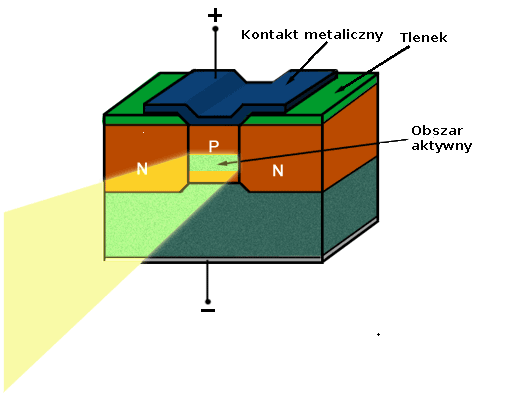
\includegraphics[width=0.7\textwidth]{./obrazki/rys-eel.png}
 % rys-eel.gif: 0x0 pixel, 300dpi, 0.00x0.00 cm, bb=
\end{center}
\caption{Budowa diody laserowej emitującej światło poprzecznie (na podstawie: \cite{rys-laserki})}
\label{rys-eel}
\end{figure}


\begin{figure}
\begin{center}
 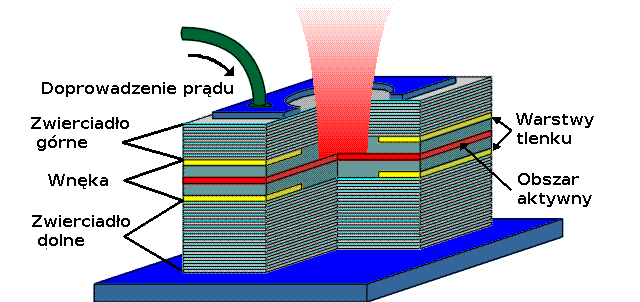
\includegraphics[width=0.8\textwidth]{./obrazki/rys-vcsel.png}
 % rys-eel.gif: 0x0 pixel, 300dpi, 0.00x0.00 cm, bb=
\end{center}
\caption{Budowa diody z pionową wnęką rezonansową (na podstawie: \cite{rys-laserki})}
\label{rys-vcsel}
\end{figure}

Taka konstrukcja diody laserowej ma jednak liczne wady. Są to:
\begin{itemize}
 \item Wysoki koszt - producja wymaga nietypowego procesu, jakim jest dokładna obróbka bocznych krawędzi struktury
 \item Duży prąd progowy dla laserowania, przez co niska sprawność - ze względu na relatywnie dużą powierzchnię złącza.
 \item Długi obszar aktywny (od kilku do kilkuset $\mathrm{\mu m}$) sprawia, że laser może pracować w wielu modach podłużnych.
 \item Astygmatyzm emitowanego światła, ze względu na asymetryczne wymiary obszaru aktywnego.
 \item Wrażliwość na pasożytnicze sprzężenia optyczne ze względu na niską dobroć rezonatora
\end{itemize}

Wolna od powyższych wad jest konstrukcja lasera o emisji powierzchniowej z pionową wnęką rezonansową (VCSEL -\textit{Vertical Cavity Surface Emitting Laser}). Jego budowa jest przedstawiona na rysunku \ref{rys-vcsel}. W takim laserze prąd przepływa przez obszar mający postać punktu, nie paska, a emisja światła zachodzi w kierunku powierzchni kryształu. W takiej sytuacji nie jest możliwe stworzenie rezonatora na samych jedynie powierzchniach kryształu. Jako że tworzenie warstw równolegle do powierzchni półprzewodnika, o precyzyjnie regulowanej grubości, nie nastręcza żadnych technologicznych trudności, zwierciadła są wykonane jako tzw. rozproszone zwierciadła Bragga, czyli wiele naprzemiennych warstw substancji o różnych współczynnikach załamania. Dla określonej długości fali pomiędzy falami odbitymi od kolejnych granic ośrodków zachodzi konstruktywna interferencja, co pozwala takiej strukturze bardzo efektywnie odbijać światło, pełniąc przy okazji rolę filtra pasmowego, umożliwiając wzmocnienie tylko jednej długości fali. Typowe wartości współczynnika odbicia to $99\%$ dla zwierciadła przedniego i $99{,}9\%$ dla tylnego. Tak utworzony rezonator, optyczny ma szereg wyróżniających cech. Jest bardzo krótki, przez co mody są bardzo dobrze rozseparowane, co bardzo ułątwia pracę w jednym modzie poprzecznym. Ze względu na bardzo wysoką dobroć rezonatora, pomimo niewielkiej jego długości, udaje się uzyskać niewielką szerokość linii. Wysoka dobroć sprawia również, że lasery VCSEL są praktycznie niewrażliwe na pasożytnicze sprzężenia optyczne.
Ze względu na warstwową budowę, obszar aktywny ma emisję poprzeczną, co pozwala laserom VCSEL emitować światło o praktycznie idealnym rozkładzie przestrzennym ($\mathrm{M^2} \cong 0$). Wysoka gęstość prądu przepływająca przez punktowy obszar aktywny pozwala uzyskać niski prąd progu laserowania, co sprawia, że lasery VCSEL są jednymi z najbardziej wydajnych źródeł światła jakie dotychczas wynaleziono. Brak konieczności obróbki krawędzi bocznych pozwala testować gotowe struktury jeszcze na waflu (krysztale bazowym), jak również oddzielać je od siebie standardowymi metodami, tj. przez cięcie piłą. 

Lasery VCSEL mają również swoje wady. Mała długość rezonatora skutkuje poszerzeniem linii. Jest ona na ogół kilkanaście razy szersza od linii generowanej przez lasery z emisją boczną. Niewielki rozmiar i przez to bardzo wysoka gęstość prądu w obszarze ograniczają maksymalną moc do (na ogół) kilku miliwatów, podczas gdy diody z emisją boczną uzyskują moce rzędu setek miliwatów. Problemem jest dodatkowo skłonność laserów VCSEL do pracy wielomodowej.

\section{Ten tytuł sen z powiek mi spędza}

\emph{Ten i poprzedni rozdział powinny mieć wg. mnie wspólny tytuł typu ,,Zarys czegośtam" na kształt ,,Wstępu teoretycznego", tyle że bez teorii.}

\subsection{Stabilizacja długości fali}

Częstotliwość $\nu$ przejścia $D1$ w rubidzie wynosi $3{,}77 \cdot 10^{14}~
\mathrm{Hz}$, podczas gdy szerokość pojedynczej linii absorpcyjnej,
nawet poszerzonej Dopplerowsko, jest rzędu $10^8~\mathrm{Hz}$. Oznacza to, że 
chcąc utrzymać długość fali dostrojoną do przejścia atomowego,
trzeba zapewnić dokładność względną rzędu $10^{-7}$. Oznacza to na przykład, że przy założeniu zależności temperaturowej $0{,}05 ~\mathrm{nm/K}$ (tak zmierzono), temperatura struktury lasera musi być ustalona z dokładnością do $2~\mu K$. Zapewnienie,
że nie tylko temperatura, ale inne czynniki, jak prąd diody i efety jej 
starzenia się, będą niezminne przez długi okres czasu, jest zadaniem 
praktycznie niemożliwym.

Jeśli więc tak dokładna stabilność długości fali jest wymagana, trzeba uciec się do aktywnej 
stabilizacji, w której koryguje się długość fali na bieżąco, zamiast utrzymywać 
wszystkie parametry na stałym poziomie.
Taka stabilizacja może dojść do skutku, jeżeli istnieje możliwość strojenia 
lasera w zakresie zawierającym linię absorpcyjną, a detekcja tej absorpcji pozwala stwierdzić, czy laser jest dostrojony, czy nie.

\begin{figure}
 \subfigure[]{
\includegraphics[width=0.3\textwidth]{./obrazki/lock_g1.eps}
\label{fig:lock1a}
}
\subfigure[]{
\includegraphics[width=0.5\textwidth]{./obrazki/lock_g2.eps}
\label{fig:lock1b}
}
\caption{Bezpośrednia metoda stabilizacji. a) Sygnał absorpcji, linią przerywaną zaznaczono poziom odniesienia. b) Sygnał błędu. Na zielono zaznaczony zakres dopuszczalnych odchyleń.}
\label{fig:lock1}
\end{figure} 


Pierwszy, najprostszy, sposób stabilizacji polega na takiej korekcji długości 
fali, by absorpcja w ośrodku pozostawała ciągle taka sama.
Metoda jest zilustrowana wykresem na rysunku \ref{fig:lock1}. Jeśli absorpcja 
jest zbyt duża, laser przestrajany jest ,,w lewo'', a jeśli zbyt mała, ,,w 
prawo``.
W efekcie, powoduje to stabilizację długości fali do lewej strony linii absorpcyjnej.
Jeśli zmieniony zostanie kierunek korekty (z lewa na prawo), uzyskamy stabilizację do prawej strony linii.

Metoda ta ma ewidentną zaletę, jaką jest prostota, oraz brak potrzeby dodatkowego zaburzania (tj. modulacji) długości fali.
Niestety, ma ona również szereg wad. Pierwszą z nich jest niemożliwość ustawienia się na środku linii. Jak widać na
rysunku \ref{fig:lock1}, zakres poprawnej pracy (zamalowany na zielono), jest silnie asymetryczny -- rozciąga się 
bez końca w lewo i jedynie krótki odcinek na prawo względem punktu stabilizacji. Warto zauważyć, że sytuacja jest tu tym gorsza, im
bliżej środka linii chcemy się ustawić.

\begin{figure}
 \subfigure[]{
\includegraphics[width=0.5\textwidth]{./obrazki/lock_g3.eps}
\label{fig:lock2a}
}
\subfigure[]{
\includegraphics[width=0.5\textwidth]{./obrazki/lock_g4.eps}
\label{fig:lock2b}
}
\caption{Przypadek, gdy absorpcja i wahania mocy lasera tego są samego rzędu. a) Sygnał absorpcji i ustalony poziom odniesienia. b) Sygnał błędu. Tylko zielony umożliwia stabilizację. }
\label{fig:lock2}
\end{figure} 


Dużo bardziej poważną wadą jest jednak ogromna wrażliwość na fluktuacje mocy lasera, jeżeli absorpcja w komórce jest niewielka.
Rysunek \ref{fig:lock2} ilustruje ten problem. Jeśli, jak na rysunku, absorpcja w ośrodku jest na poziomie 2\%, poziom odniesienia
należy ustawić na 99\% transmisji. Oznacza, to, że jeśli moc lasera zmini się, albo do detektora dotrze światło zewnętrzne o wartości
zaledwie 1\% przechodzącej wiązki, stabilizacja stanie się niemożliwa.

\begin{figure}

\includegraphics[width=\textwidth]{./obrazki/lock_g5.eps}
\caption{Stabilizacja z użyciem detekcji fazoczułej.}
\label{fig:lock3}
\end{figure} 

Istnieje jednak metoda stabilizacji wolna od tych wad.
Polega ona na ciągłej zmianie długości fali w kontrolowany sposób i obserwacji zmian transmisji tym wywołanych. (patrz rysunek \ref{fig:lock3})

 Długość fali lasera jest podmodulowana, czyli periodycznie zmienia się w czasie. Ilustrują to niebieskie, pionowe sinusoidy na rysunku. Ich amplituda odpowiada amplitudzie wahań długości fali.
  Zależnie od położenia względem środka krzywej rezonansowej, zmiana absorpcji wywołana modulacją (czarne, poziome sinusoidy) może mieć
 różną amplitudę, i co najważniejsze, być w fazie, lub przeciwfazie do modulacji.
  Amplituda zmian absorpcji jest więc de facto pochodną krzywej absorpcyjnej po długości fali (czerwona krzywa). 
  Ma ona antysymetryczny przebieg względem środka linii, a z jej znaku (pod warunkiem, że w otoczeniu jest tylko jedna linia absorpcyjna)
 można jednoznacznie odczytać, w którą stronę powinna nastąpić korekta.
 
 Taka metoda stabilizacji pozwala całkowicie wyeliminować zależność długości fali od fluktuacji mocy (jak na rys. \ref{fig:lock2})  i maksymalnie zminimalizować wpływ zmiennej głębokości linii absorpcyjnych (zależność ta znika całkowicie w punkcie, gdzie sygnał błędu jest zerowy, czyli na środku linii).

Zmiana absorpcji jest proporcjonalna (przez czynnik równy pochodnej absorpcji dla bieżącej długości fali) do wielkości zmiany długości fali. Oznacza to, że gdy dłogość fali jest zmieniana harmonicznie, jak $\cos \omega t$, absorpcja zmienia się także harmonicznie, co można zapisać jako $A \cos \omega t$. Dokładne wyznaczenie amplitudy (parametru $A$)
umożliwie technika nazywana detekcją fazoczułą.

\subsection{Magnetorotacja i nieliniowy efekt Faradaya}

Fotony, będąc absorbowane przez atomy w próbce, przeprowadzją atomy ze stanu podstawowego do wzbudzonego.
Zapis stanów w bazie $|F,m_F\rangle$ pozwala na przejrzystą analizę możliwych przejść.
W szczególności, niektóre przejścia między stanami są wykluczone ze względu na zasady zachowania: momentu pędu i parzystości funkcji falowej. Schemat poziomów dla rubidu przedstawia rys. (\ref{poziomyRb})


\begin{figure}
\begin{center}
 \includegraphics[width=0.8\textwidth]{./obrazki/figure3.JPG}
 % rys-eel.gif: 0x0 pixel, 300dpi, 0.00x0.00 cm, bb=
\end{center}
\caption{Schemat poziomów energetycznych dla przejścia D1 w rubidzie}
\label{poziomyRb}
\end{figure}

Poszczególne polaryzacje światła mogą dokonać następującej zmiany stanu atomów:
\begin{center}
\begin{description}
\item[polaryzacja $\sigma_+$] zwiększa $m_F$ o 1,
\item[polaryzacja $\sigma_-$] zmniejsza $m_F$ o 1,
\item[polaryzacja $\pi$] pozostawia $m_F$ bez zmian.
\end{description}
\end{center}

Oświetlenie atomów światłem o polaryzacji $\sigma_+$ (polaryzacja $\sigma$--wiązka równoległa do linii pola magnetycznego) powoduje przepompowanie populacji do stanu o $m_F$ maksymalnym ($m_F$=+1). Podobnie, oddziaływanie ze światłem $\sigma_-$ będzie prowadzić do przepompowania atomów do stanu o $m_F=-1$. Stany te nazywamy stanami ciemnymi (dla zadanej polaryzacji światła).

Dla światła o polaryzacji liniowej $\sigma$ również występuje stan ciemny, postaci $$\psi_d=\frac{1}{\sqrt{2}} (|g,+\rangle-|g,-\rangle).$$ Takie uporządkowanie ośrodka, w którym powyższy stan jest silnie obsadzony, nazywamy orientacją, ze względu na zerowy wypadkowy moment magnetyczny. Ośrodek, w którym jest wytworzona taka orientacja wykazuje anizotropię współczynnika załamania, ponieważ dla jednej z polaryzacji liniowych występuje stan ciemny, a polaryzacja do niej prostopadła jest absorbowana. Ośrodek może być więc rozpatrywany jako płytka falowa. Nie skręca jednak płaszczyzny polaryzacji wiązki pompującej, ponieważ ta jest współliniowa z jednym z jej azymutów.

W polu magnetycznym momenty magnetyczne, jak również wytworzona orientacja, obracają się z częstością Larmora $\omega_L$. Obrót ,,płytki falowej" powoduje skręcenie polaryzacji padającego światła.

Obrót powoduje jednak, że stan dotychczas ciemny, zaczyna absorbować światło. Światło przeciwdziała obrotowi, próbując odtworzyć alignment przez ciągłe pompowanie optyczne.

Przy stałej szybkości obrotu (polu magnetycznym $\vec B$), orientacja ulega więc odchyleniu od początkowej osi w stopniu tym większym, im słabsza wiązka pompująca (w zakresie małych kątów). Osłabienie wiązki pompującej powoduje jednak osłabienie orientacji, ponieważ bez pompowania uporządkowanie zanika. Innymi słowami, sytuacje skrajne to silne uporządkowanie, ale niewielkie odchylenie osi anizotropii od płaszczyzny polaryzacji światła oraz duże odchylenie ale niski stopień uporządkowania atomów. W obydwu tych sytuacjach płaszczyzna polaryzacji ulega słabemu skręceniu.

Można wykazać \cite{srivansan}, że istnieje optymalne natężenie wiązki padającej, związane z optimum parametru:
\begin{equation}
\kappa=\frac{\Omega_R}{\Gamma\gamma} \; ,
\end{equation}
gdzie $\Omega_R=\frac{|d \cdot E|}{\hbar}$ to częstość Rabiego, odpowiadająca sile pompowania ($d$ to moment dipolowy przejścia a $E$ natężenie pola padającego światła), a $\Gamma$ i $\gamma$ -- natężenia opisywanych procesów dekoherencji.

Zjawisko jest nazywane nieliniowym efektem Faradaya, ponieważ skręcenie polaryzacji światła zależy (nieliniowo) od mocy padającego światła.

Opisywany efekt skręcenia płaszczyzny polaryzacji światła zachodzi w otoczeniu $|\vec B|=0$. Przy obserwacji zależności skręcenia płaszczyzny polaryzacji światła przez ośrodek od pola $\vec B$, powinna być widoczna antysymetryczna zależność ($B=0\rightarrow$ zerowe skręcenie).

 Zastosowanie modulacji światła zwiększa zakres mierzalnych pól magnetycznych. Częstość modulacji musi być taka, żeby w ciągu okresu przebiegu modulującego alignment atomowy obrócił się o wielokrotność kąta $\pi$. 
Podczas obrotu w polu magnetycznym występuje także odchylanie płaszczyzny polaryzacji, pod warunkiem ciągłego odtwarzania alignmentu. Przy oświetlaniu ośrodka impulsami światła o częstości $\Omega_m$ rezonans będzie więc występować przy częstości
\begin{equation}
\Omega_m=\frac{2 \omega_l}{n} \; ,
\end{equation}
gdzie $n=1,2,3$ to ilość półobrotów jakie wykona alignment w cyklu modulacji. Absorpcja będzie wtedy najniższa, ponieważ światło będzie napotykać zawsze takie samo, napompowane, ustawienie atomów.

W rezonansie, przy częstości modulacji $\Omega_m$, orientacja atomów jest najsilniesza. Oznacza to największą amplitudę wahań płaszczyzny polaryzacji światła. Zależność amplitudy wahania płaszczyzny polaryzacji światła
od częstotliwości modulacji daje się opisać krzywą rezonansową \ref{krzywa}. Obserwując oprócz amplitudy wahania płaszczyzny polaryzacji także jej zależność fazową względem przebiegu modulującego, tj. składową w fazie i w kwadraturze, można wyodrębnić część absorbcyjną (symetryczną względem częstości rezonansowej) i elastyczną (asymetryczną).

Krzywa rezonansowa (Lorentza) jest rozwiązaniem oscylatora harmonicznego z wymuszeniem i ma postać:
\begin{equation}
c(\omega)=\frac{\Gamma  \Omega  \left(\Gamma  \omega -i \left(\Omega ^2-\omega ^2\right)\right)}{\Gamma ^2 \omega ^2+\left(\Omega ^2-\omega ^2\right)^2} \; ,
\label{krzywa}
\end{equation}

gdzie $\Omega$ -- częstość rezonansowa (zazwyczaj na osi $x$) i $\Gamma$ -- szerokość rezonansu.\\

\begin{itemize}
 \item O co chodzi ze stab. na 1H i pomiarem na 2H
 \item Po co komórki mają pokrycie parafinowe / gaz. Co to robi za różnicę.
\end{itemize}


\pagebreak

\section{Zbudowana aparatura}

\subsection{Użyta dioda}

\begin{figure}
\begin{center}
 \includegraphics[width=0.8\textwidth]{./obrazki/vcsel_struktura.png}
 % rys-eel.gif: 0x0 pixel, 300dpi, 0.00x0.00 cm, bb=
\end{center}
\caption{Użyta dioda laserowa (Vixar Inc.)}
\label{struktura}
\end{figure}

Do wykonania pomiarów została użyta dioda wyprodukowana przez firmę $Vixar$, o oznaczeniu
W strukturze, przedstawionej na rys. (\ref{struktura}), producent umieścił cztery identyczne złącza. Niestety, po i ch sprawdzeniu i wybraniu najlepszej z nich, z sobie tylko znanych powodów zdecydował się odłączyć pozostałe trzy.

W trakcie pomiarów dioda uległa uszkodzeniu. Wycieczka na AGH zaowocowała przyłączeniem pozostałych struktur, który okazały się działać bardzo dobrze. PODZIĘKOWAĆ PANU IDZIKOWI Z KOLEGAMI.

Parametry jej pracy to:
\begin{center}
\begin{tabular}{ll}
Prąd maksymalny & $4 ~\mathrm{mA}$\\
Próg laserowania & $0{,}6~\mathrm{mA}$\\
Maksymalny prąd pracy jednomodowej & $1{,}6~\mathrm{mA}$\\
Moc nominalna & $150~\mathrm{\mu }W$\\
Moc przy pracy jednomodowej & $60~\mathrm{\mu W}$\\
Szerokość linii & $100~\mathrm{MHz}$\\
Stała strojenia prądem & COŚCOŚTAM\\
Stała strojenia temperaturą & $0.05 ~\mathrm{nm/{}^{\circ}C}$\\
Optymalny prąd & $1{,}5 ~\mathrm{mA}$\\
Optymalna temperatura & $26~\mathrm{ {}^{\circ}C}$ \\
Obudowa & TO-46 z pięcioma nogami
\end{tabular}
\end{center}


\subsection{Układ zasilania}

Na rysunku (\ref{sch-psu}) przedstawiony jest schemat pierwszego z układów elektronicznych użytych w pracy -- zasilacza diody. Jego zadaniem jest zasilanie diody laserowej prądem o regulowanej, stabilnej w czasie wartości i jak najniższej fluktuacji (szumie). Zbyt duży poziom szumu obecny w niededykowanym zasilaczu znanej firmy był jednym z powodów zaprzestania prac z laserem o emisji powierzchniowej, co jest opisane w pracy mgr. Justyny Mech \cite{mgrJustynaMech}.

Działanie układu najwygodniej opisać od strony lasera. Z dodatniego napięcia zasilającego, przez tranzystor \textit{Q2} i rezystor pomiarowy \textit{R5}, prąd płynie do anody diody laserowej, dołączoną do złącza P1. Katoda diody jest dołączona do masy, co czyni diodę bardziej odporną na przepięcia i przypadkowe zwarcie niż w sytuacji, gdyby obydwa końce były ,,pływające``.  
Właściwe źródło prądowe jest bardzo proste -- formuje je rezystor R3 zasilając z kondensatora C1 bazę tranzystora \textit{Q2}. Tranzystor Q1 i rezystor R1 stanowią obwód zabezpieczający i można je pominąć przy analizie normalnej pracy układu. Prąd kolektora Q2 jest już właściwym prądem diody laserowej. Warto zaznaczyć, że w tym układzie nie występuje praktycznie żaden szum nadmiarowy -- pod wpływem stałego napięcia na kondensatorze przez rezystor o sporej wartości przepływa stały prąd, który jest praktycznie idealnie bezszumnie wzmacniany przez pojedynczy tranzystor. Wysoki opór różniczkowy kolektora tranzystora \textit{Q2}, sprawia, że układ stanowi dobre źródło prądowe, tj. prąd nie zależy od napięcia na obciążeniu. Oczywiście, ponieważ zakładamy niezmienność napięcia na C1 oraz napięcia baza-emiter i wzmocnienia tranzystora Q2, taki obraz jest poprawny tylko dla wysokich częstotliwości. Długoczasową stabilizację prądu zapewnia wzmacniacz U1, który działa w układzie wzmacniacza pomiarowego, zapewniając na swoim wyjściu takie napięcie, by napięcie na rezystorze pomiarowym R5 poprzez rezystory R4 i R7 równoważyło napięcie zadawane między wyjściem U2 a masą, przez rezystory  R8 i R11.
Dodatkowe rezystory R9 i R10 pozwalają w niewielkim zakresie podmodulować prąd diody, napięciem podanym przez złącze P2.
Napięciu 1V na wyjściu U2 odpowiada 1 mA prądu płynącego przez diodę.

Układ U2 stanowi filtr dolnoprzepustowy, o niskiej częstości odcięcia (rzędu 10 Hz), eliminujący szum i trzaski z napięcia pochodzącego z potencjometru PR1, którym ustawia się prąd. Zwora JP1 pozwala wybrać pomiędzy zakresem $0-3{,}5$~mA a 0-7~mA.

Napięcie wzorcowe, dostarczane na nóżkę 3 potencjometru pochodzi z diody Zenera D1. Dioda ta to wysoce stabilna dioda o tzw. strukturze zagrzebanej, zintegrowana wraz z termostatem. Decyduje to o doskonałej stabilności cieplnej ($0.5~\mathrm{ppm}/{}^{\circ}C$) i długoczasowej.  Wzmacniacz U3 zasila diodę stałym prądem, zadawanym jej własnym napięciem Zenera. Jest on zasilany inaczej niż pozostałe, pojedynczym napięciem. Uniemożliwia to ,,zatrzaśnięcie'' się układu na napięciu przewodzenia diody (ujemnym) zamiast na napięciu Zenera (dodatnim). 

\begin{figure}
\begin{center}
 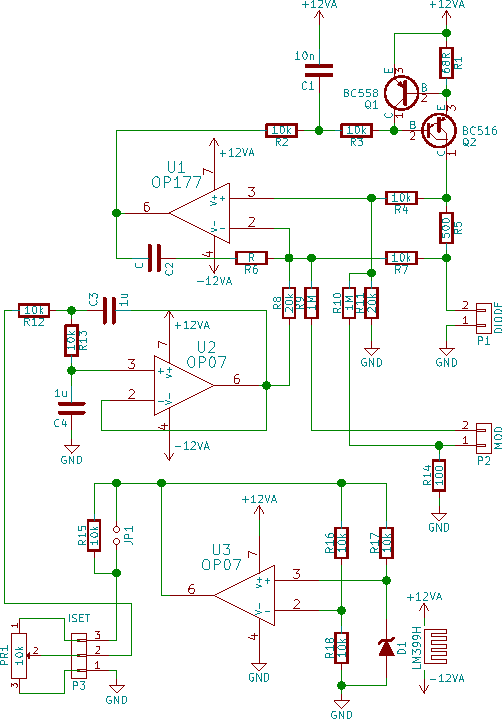
\includegraphics{./obrazki/VcselPSU.pdf}
 % rys-eel.gif: 0x0 pixel, 300dpi, 0.00x0.00 cm, bb=
\end{center}
\caption{Schemat zasilacza diody}
\label{sch-psu}
\end{figure}

\subsection{Układ modulacji}

Po zbadaniu modułu zasilania, kolejnym krokiem było zbadanie, jak szybko można modulować prąd diody, co ma na celu szybką zmianę długości fali. Jako że te diody służą do transmisji danych z prędkością kilku Gb/s, modulacja częstościami na poziomie kilkuset MHz powinna być realna. 

Elektryczny schemat zastępczy diody laserowej przedstawiony jest na rysunku \ref{sch-mod1}. 
\begin{figure}
\begin{center}
 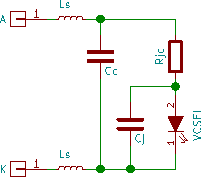
\includegraphics{./obrazki/sch_mod1.pdf}
 % rys-eel.gif: 0x0 pixel, 300dpi, 0.00x0.00 cm, bb=
\end{center}
\caption{Uproszczony schemat zastępczy diody laserowej}
\label{sch-mod1}
\end{figure}
Na jego podstawie można założyć, że na dynamikę modulacji prądu, tj. jej maksymalną szybkość oraz przesunięcie fazowe mają wpływ jedynie wartości pasożytniczych pojemności i indukcyjności, oraz opór wewnętrzny diody. Konsekwencją tego założenia jest możliwość kompensacji wpływu pasożytniczych elementów poprzez manipulacje jedynie impedancją źródła sygnału, w efekcie uzyskując płaską zależność amplitudy modulacji światła od częstotliwości.
Dla najwyższych częstotliwości (gigaherce) model ten może przestawać odzwierciedlać rzeczywidość, ze względu na wpływ skończonego czasu potrzebnego do osiągnięcia równowagi między pompowaniem a emisją promieniowania z rezonatora. Poczyniono nieme założenie, że modulacja jasności jest równoznaczna modulacji długości fali. Jest ono spełnione, jeśli procesy optyczne (pompowanie i relaksacja) zachodzą znacznie szybciej niż zmiany prądu w strukturze.

Zbudowano układ umożliwiający szybką modulację prądu sygnałem dostarczanym standardowym kablem koncentrycznym ze złączem SMA.

Zadania układu są następujące:
\begin{itemize}
 \item Dopasowanie impedancji wejściowej do kabla ($50~\Omega$).
 \item Osłabienie sygnału (docelowe zmiany prądu mają być rzędu $\mu A$)
 \item Uzyskanie płaskiej charakterystyki modulacji światła od częstotliwości przy stałym poziomie sygnału wejściowego
\end{itemize}

Ostatni cel został osiągniety głównie metodą prób i błędów. Opór wewnętrzny diody (przy prądzie pracy) został zmierzony jako $61~ \Omega$.
Docelowy układ przedstawia rysunek \ref{sch-mod1}. Na płytce znajdują się diody zabezpieczające (specjalne diody zabezpieczające przed elektrostatycznymi wyładowaniami, bardzo szybkie i o niskim prądzie upływu) oraz złącza doprowadzające prąd z zasilacza i sygnał modulujący z generatora. Pojemność kondensatora kompensacyjnego został dobrana tak, by uzyskać możliwie płaską charakterystykę modulacji. Zależność odpowiedzi częstotliwościowej od jego pojemności znajduje się na rysunku \ref{wyk-mod}.

\begin{figure}
\begin{center}
 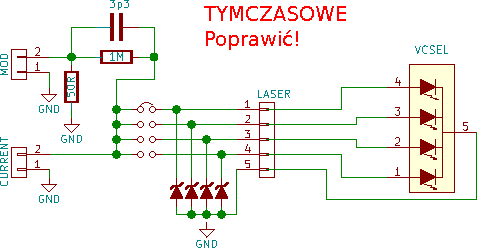
\includegraphics{./obrazki/dings.pdf}
 % rys-eel.gif: 0x0 pixel, 300dpi, 0.00x0.00 cm, bb=
\end{center}
\caption{Schemat płytki znajdującej się przy diodzie laserowej}
\label{sch-mod}
\end{figure}

\begin{figure}
\begin{center}
 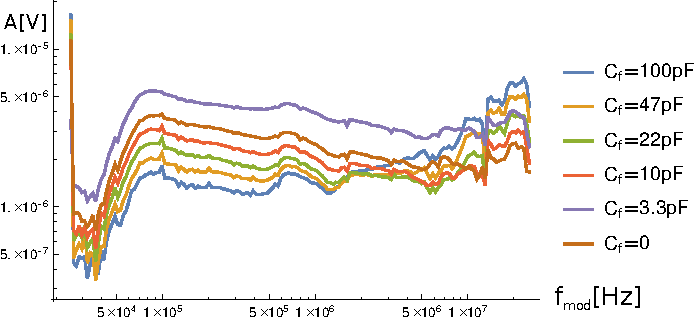
\includegraphics[width=0.8\textwidth]{./obrazki/bw.pdf}
 % rys-eel.gif: 0x0 pixel, 300dpi, 0.00x0.00 cm, bb=
\end{center}
\caption{Zależność charakterystyki częstotliwościowej modulacji od pojemności kondensatora kompensacyjnego}
\label{wyk-mod}
\end{figure}

\subsection{Cyfrowe strojenie}

Aby uprościć proces dostrajania do linii po uruchomieniu lasera, opracowano układ pozwalający na sterowanie prądem lasera z programu uruchomionego na komputerze.
Umożliwia on rejestrację zależności absorpcji w komórce od prądu, detekcję linii absorpcyjnych, a później automatyczne dostrojenie lasera do wybranej linii.

Moduł strojenia podłącza się zamiast potencjometru regulacji prądu. Układ składa się z mnożącego przetwornika cyfrowo-analogowego, o rozdzielczości 16 bitów, mikrokontrolera i układu konwertera USB $\leftrightarrow$ RS-232. W trakcie testów stwierdzono, że rozdzielczość przetwornika jest więcej niż wystarczająca (linie absorpcyjne mają szerokość ok. 100LSB przetwornika), a układ jest znacznie stabilniejszy od potencjometru (dryf i szum są znacznie mniejsze niż 1LSB). Dane między modułem a komputerem wymieniane są za pośrednictwem złącza USB.

Moduł jest sterowany przy pomocy programu na komputer PC. Jest on napisany w języku Python, z wykorzystaniem interfejsu graficznego Qt. Kod źródłowy programu można znaleźć w \url{https://github.com/ccucumber/laserscan}. Okno główne programu przedstawione jest na rysunku \ref{scr-main}.

\begin{figure}
\begin{center}
 \includegraphics[width=0.8\textwidth]{./obrazki/scr_main.png}
 % rys-eel.gif: 0x0 pixel, 300dpi, 0.00x0.00 cm, bb=
\end{center}
\caption{Główne okno programu}
\label{scr-main}
\end{figure}


Po lewej stronie okna programu znajduje się szereg przycisków, oferując następujące możliwości:

\begin{itemize}
 \item Uruchomienie skanowania lasera, w zakresie od ,,Start`` do ,,Stop``, z krokiem ,,Step''. Absorpcja jest przedstawiana na wykresie, a postęp skanowania jest widoczny na pasku postępu.
 \item Zapis i odczyt zmierzonych wartości absorpcji do/z pliku.
 \item Automatyczne szukanie linii absorpcyjnych
 \item Dostrojenie do wybranej z listy, znalezionej w poprzednim kroku pozycji linii absorpcyjnej.
\end{itemize}


\begin{figure}
\begin{center}
 \includegraphics[width=0.8\textwidth]{./obrazki/scr_anal.png}
 % rys-eel.gif: 0x0 pixel, 300dpi, 0.00x0.00 cm, bb=
\end{center}
\caption{Okno szukania linii absorpcyjnych}
\label{scr-anal}
\end{figure}

Po naciśnięciu przycisku ,,Analyze`` program wyświetla okno pokazane na \ref{scr-anal}.
Aby uzyskać ten efekt, wykonywane są następujące operacje:
\begin{enumerate}
 \item Następuje odcięcie składowej stałej przez dopasowanie i odjęcie wielomianu niskiego stopnia.
 \item Przebieg jest wygładzany przez uśrednienie kilku sąsiednich próbek
 \item Znajdowane i zaznaczane na wykresie są linie absorpcyjne o dostatecznej głębokości względem aktualnie zarejestrowanego maksimum absorpcji
\end{enumerate}





\subsection{Stabilizacja długości fali}

Po dostrojeniu lasera zachodzi konieczność ciągłej korekty długości fali, tak by pozostać na linii absorpcyjnej.

Jest to realizowane metodą opisaną w następnym rozdziale, na podstawie sygnału z wzmacniacza fazoczułego. %KTÓRYM ROZDZIALE?
Jako że sygnał ze wzmacniacza fazoczułego jest proporcjonalny do odstrojenia lasera od zadanej długości fali, koncepcja układu stabilizującego jest prosta.
Jest to typowy regulator proporcjonalno-całkująco-różniczkujący. Schemat jest przedstawiony na rysunku \ref{sch-pid}.

\begin{figure}
\begin{center}
 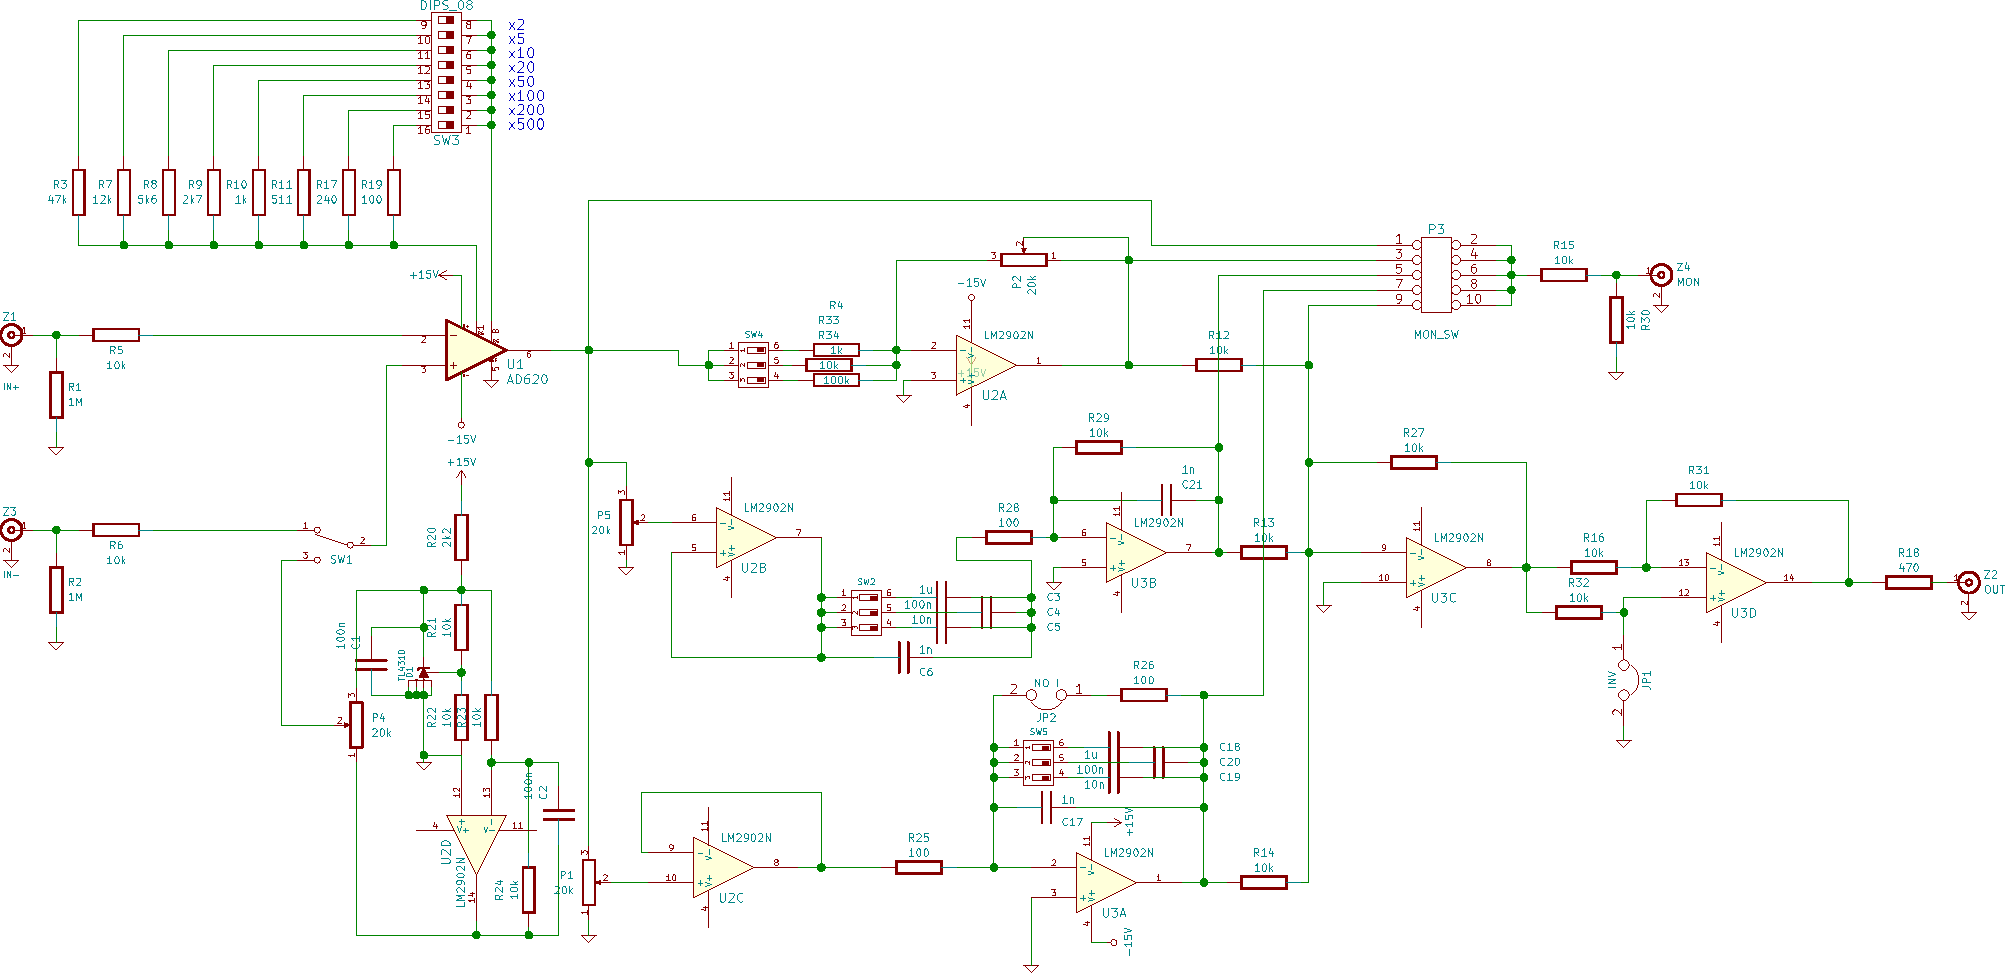
\includegraphics[scale=0.58, angle =90 ]{./obrazki/pidella.pdf}
 % rys-eel.gif: 0x0 pixel, 300dpi, 0.00x0.00 cm, bb=
\end{center}
\caption{Schemat regulatora PID}
\label{sch-pid}
\end{figure}

Układ posiada dwa wejścia, przy czym jedno z nich może być odłączone i zastąpione przez potencjał ustawiany potencjometrem P4. Przełącznik SW3 ustawia wstępne wzmocnienie.
Dalej sygnał jest rozdzielany do trzech członów -- od góry: proporcjonalnego, różniczkującego i całkującego.
Wzmocnienie pierwszego ustalane jest skokowo przez SW4 i płynnie przez potencjometr P2, analogicznie ustawiana jest stała czasowa członu różniczkującego (SW2 i P5) i całkującego ( SW5, P1). Zwora JP2 wyłącza człon całkujący na czas wstępnego dostrojenia.
Sygnały z trzech członów są sumowane przez wzmacniacz U3C. Zwora JP1 pozwala zmienić polaryzację sygnału wyjściowego na przeciwną.

Dodatkowe wyjście Z4 pozwala na monitorowanie sygnału wybranego zworą P3.

\subsection{Polarymetr wraz z układem detekcji}

Laser, dostrojony do pożądanego przejścia atomowego, oddziałuje z atomami rubidu w komórce.
Skutkiem tego oddziaływania jest osłabienie wiązki -- absorpcja oraz rotacja płaszczyzny polaryzacji światła.
Precyzyjny pomiar powyższych ma kluczowe znaczenie dla dokładności magnetometrii optycznej.

\begin{figure}
\begin{center}
 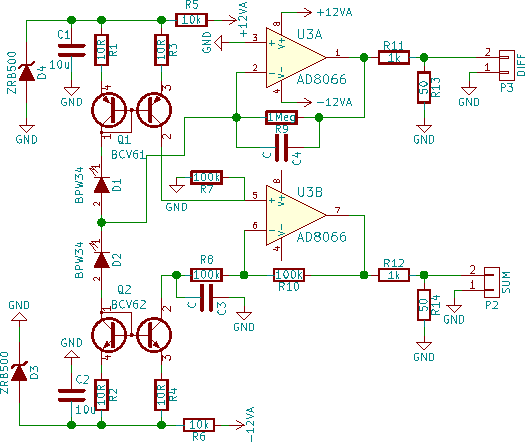
\includegraphics{./obrazki/polarymetr.pdf}
 % rys-eel.gif: 0x0 pixel, 300dpi, 0.00x0.00 cm, bb=
\end{center}
\caption{Schemat polarymetru}
\label{sch-mod}
\end{figure}

Polarymetr posiada dwie fotodiody i wytwarza dwa sygnały - o amplitudzie proporcjonalnej do różnicy i sumy natężeń światła padającego na fotodiody.
Sygnał różnicy służy do pomiaru skręcenia polaryzacji, która bezpośrednio zależy od pola magnetycznego.  Sygnał sumy pozwala zaś śledzić absorpcję w komórce, co umożliwia stabilizację lasera na linii.

Sygnał różnicy jest wytwarzany przez wzmacniacz U3A, pracujący w typowej konfiguracji transimpendancyjnej. Wzmacnia on prąd pochodzący z węzła pomiędzy fotodiodami D1 i D2.
Elementy R9 i C3 ustalają odpowiednio wzmocnienie i pasmo tego wzmacniacza.

Warto szerzej opisać to rozwiązanie. Taka konfiguracja ma szereg zalet ponad odejmowaniem sygnałów z dwóch niezależnych wzmacniaczy transimpendacyjnych z pojedynczymi fotodiodami.
Pierwszą zaletą jest mniejszy szum -- w układzie z dwoma wzmacniaczami, mimo, że sygnały są odejmowane, szumy się dodają. Drugi problem jest mniej oczywisty -- odmienna charakterystyka częstotliwościowa różnych wzmacniaczy może osłabiać tłumienie sygnału wspólnego wraz ze wzrostem częstotliwości, jako że sygnały te nie będą już przesunięte w fazie o dokładnie $180^{\circ}$, co sprawi, że zwykła absorpcja zostanie odebrana jako skręcenie. Tłumienie sygnału współbieżnego ma kluczowe znaczenie przy dokładnej detekcji niewielkich skręceń przy szerokim zakresie częstotliwości pracy.

Gdyby zastosować dwa oddzielne wzmacniacze dla fotodiod, generacja sygnału sumy nie nastręczałaby większego problemu. W układzie z różnicą ,,na drucie", konieczne jest zastosowanie dwóch luster prądowych (tranzystory podwójne Q1 i Q2) przed wzmacniaczem sumującym U3B. Górne lustro prądowe jest obciążone pojemnością nieodwracającego wejścia wzmacniacza, podczas gdy dolne lustro jest obciążone jedynie rezystancyjnie. Sytuację tę wyrównuje kondensator C3. 

Wyjścia obydwu torów są doprowadzone do dzielników 20:1, które mają na celu dopasowanie impendancji wyjściowej do kabla $50\Omega$. To z pozoru kontrowersyjne rozwiązanie nie pogarsza precyzji pomiaru -- dalsze przyrządy pomiarowe po prostu pracują na czulszym zakresie.

\section{Uruchomienie układu pomiarowego}


\section{Wyniki i jakiś opis pomiarów}




\subsection{Spektroskopia rubidu}

Aby uwiarygodnić wskazania miernika długości fali, oraz by w dalszych pomiarach móc związać kształt sygnału absorpcji w komórce (zwanego dalej spektroskopią), przeprowadzono dosyć nietypowy pomiar.
Zmierzono absorpcję w komórce dla wielu pojedynczych długości fali, zmierzonych $\lambda-$metrem. Z tych wyników skonstruowano wykres.
Wynik pomiaru z komórki o pokryciu parafinowym przedstawia rys. \ref{fig:spekpara}, a z komórki z gazem buforowym rys. \ref{fig:spekgaz}.

Widać, że w komórce z gazem buforowym nastąpiło bardzo znaczące obniżenie absorpcji (z ok. 50\% do ok. 5\%), jak również poszerzenie linii. Przesunięcie centrum linii było mniejsze od niepewności pomiaru. Dalsze pomiary wykazały, że pomimo absorpcji niższej o rząd wielkości (co utrudnia dokładny pomiar absorpcji i skręcenia), komórka z gazem buforowym lepiej sprawdziła się w pomiarach pola magnetycznego, pozwalając obserwować dużo węższe rezonanse (patrz rozdział \ref{sec:magnetorotacja}). 


\begin{figure}[h!]
\centering
 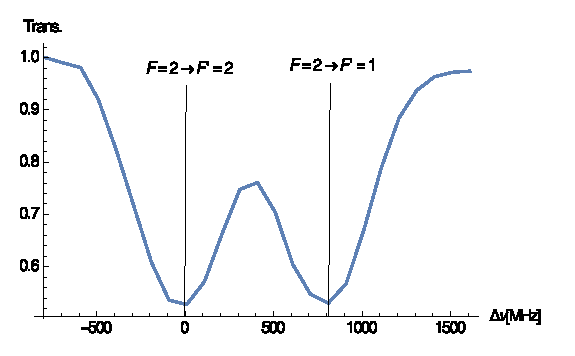
\includegraphics[width=\textwidth]{spek_para.eps}
 % front_all.svg: 1153x455 pixel, 72dpi, 40.68x16.05 cm, bb=0 0 1153 455
 \caption{Spektroskopia komórki z pokryciem parafinowym. Pomiar w $T=50^{\circ}C$}
 \label{fig:spekpara}
\end{figure}



\begin{figure}[h!]
\centering
 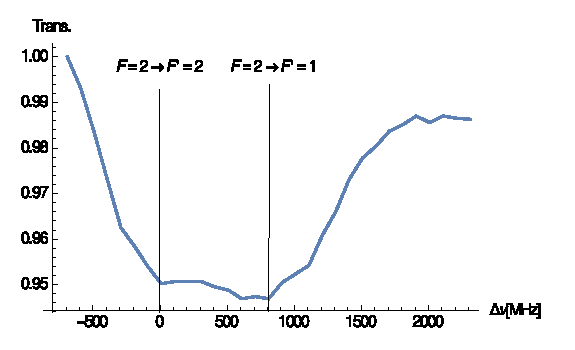
\includegraphics[width=\textwidth]{spek_gaz.eps}
 % front_all.svg: 1153x455 pixel, 72dpi, 40.68x16.05 cm, bb=0 0 1153 455
 \caption{Spektroskopia komórki z gazem. Widoczne znaczne poszerzenie linii i obniżona transmisja. $T=50^{\circ}C$}
 \label{fig:spekgaz}
\end{figure}


\section{Sygnał błędu}

Zmierzono zależność sygnału błędu stabilizacji długości fali, to jest zależność amplitudy sygnału z wyjścia wzmacniacza fazoczułego pracującego na częstotliwości modulacji (,,pierwszej harmonicznej``). Sygnał ten można interpretować jako wartość pochodnej krzywej absorpcji.

Na rysunku \ref{fig:panoda} przedstawiona jest zależność tego sygnału od amplitudy modulacji. Widać, że wraz ze wzrostem amplitudy modulacji amplituda sygnału pochodnej rośnie, ale następuje też jego poszerzenie wzdłuż osi odciętych. Jest to spowodowane tym, że przy zwiększaniu amplitudy modulacji, w pewnym momencie długości fali lasera nie można jej już traktować jako stałej, ale zachodzi jej ''rozsmarowanie" w pewnym zakresie. Efekt jest zauważalny, gdy ta szerokość staje się porównywalna z szerokością obserwowanych linii absorpcyjnych. Powyżej pewnej amplitudy modulacji nie następuje już dalszy wzrost amplitudy sygnału błędu, a jedynie jego dalsze poszerzanie. Można to dostrzec na trzech najwyższych przebiegach na rys. \ref{fig:panoda}.

Rysunek \ref{fig:panodp} przedstawia zależność sygnału błędu od mocy światła przechodzącego przez komórkę. Poszerzenie sygnału ze wzrostem mocy światła praktycznie nie występuje. Oznacza to, że moc światła nie jest zbyt wysoka, tj. nie wysyca populacji atomów w komórce.

%DODAĆ PORZĄDNE OSIE X.

\begin{figure}[h!]
\centering
 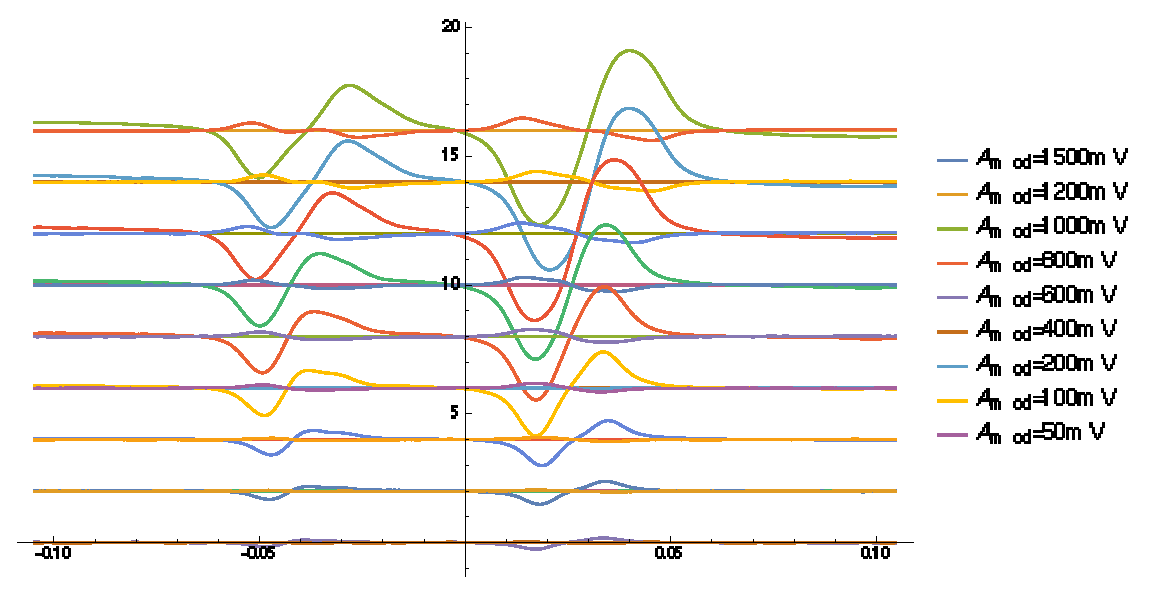
\includegraphics[width=\textwidth]{panoramy_1H_oda.eps}
 % front_all.svg: 1153x455 pixel, 72dpi, 40.68x16.05 cm, bb=0 0 1153 455
 \caption{Zależność sygnału błędu od amplitudy modulacji długości fali. $f_{mod}=101kHz, P_{las}=20 \mu W$}
 \label{fig:panoda}
\end{figure}

\begin{figure}[h!]
\centering
 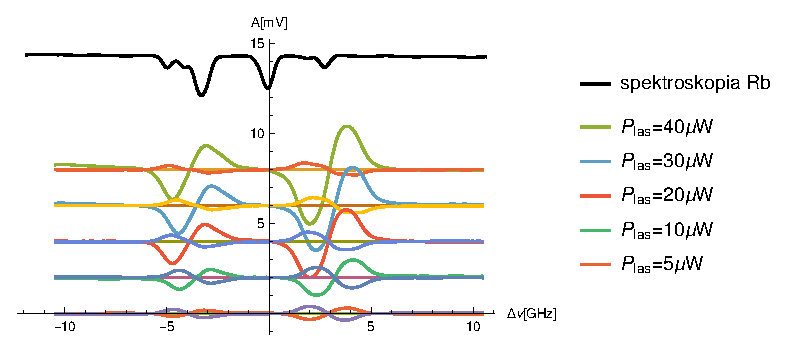
\includegraphics[width=\textwidth]{panoramy_1H_odp.eps}
 % front_all.svg: 1153x455 pixel, 72dpi, 40.68x16.05 cm, bb=0 0 1153 455
 \caption{Zależność sygnału błędu od amplitudy mocy lasera. $f_{mod}=101kHz, A_{mod}=1000mV$}
 \label{fig:panodp}
\end{figure}

\section{Magnetorotacja}
\label{sec:magnetorotacja}


Zmieniając częstotliwość modulacji długości fali lasera, możemy doprowadzić do sytuacji, gdy ta częstotliwość pokrywa się z częstotliwością precesji atomów w polu magnetycznym.
Zachodzi wtedy skręcenie polaryzacji (liniowo spolaryzowanego) światła padającego na komórkę. Skręcenie jest mierzone przez polarymetr, a jego amplitudę wyznacza wzmacniacz fazoczuły, który może mierzyć sygnał na częstotliwości modulacji oraz jej harmonicznych. Zależność amplitudy skręcenia w zależności od indukcji pola magnetycznego w komórce przedstawia rys. \ref{fig:magnetorot1}. Widać, że przebieg tej zależności ma postać krzywej rezonansowej.

\begin{figure}[h!]
\centering
 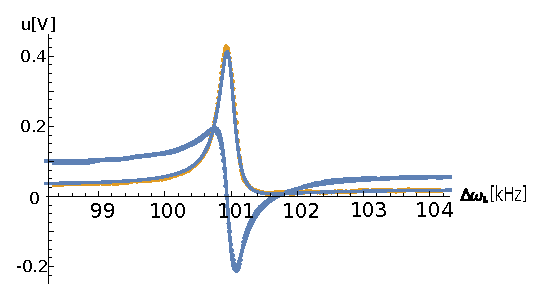
\includegraphics[width=\textwidth]{magnetorot1.eps}
 % front_all.svg: 1153x455 pixel, 72dpi, 40.68x16.05 cm, bb=0 0 1153 455
 \caption{Przykładowa zależność magnetorotacji, po detekcji fazoczułej, w zależności od pola magnetycznego. Pole magnetyczne wyrażone w jednostkach częstości Larmora dla ${}^{87} Rb$.
 $f_{mod}=101kHz, P_{las}=15 \mu W$}
 \label{fig:magnetorot1}
\end{figure}

Jednym z podstawowych celów niniejszej pracy była weryfikacja parametrów magnetorotacji, którą można uzyskać przez interakcję światła ze zbudowanego lasera z atomami.
Parametrami charakteryzującymi taki rezonans są jego  szerokość -- węższy rezonans pozwala dokładniej wyznaczyć pole magnetyczne, oraz amplituda -- większa również pozwala dokładniej mierzyć pole (przez poprawę stosunku sygnału do szumu).

Na rysunku \ref{wykresikioda} znajduje się zależność szerokosći i amplitudy sygnału magnetorotacji od amplitudy modulacji. Widać, że zbyt duża amplituda modulacji powoduje zmniejszenie skręcenia. Jest to związane z tym, że przy zbyt szerokiej modulacji światło jest przez coraz dłuższy ułamek okresu modulacji odstrojone od profilu absorpcji atomów. 

\begin{figure}[h!]
\centering
\subfigure[]{
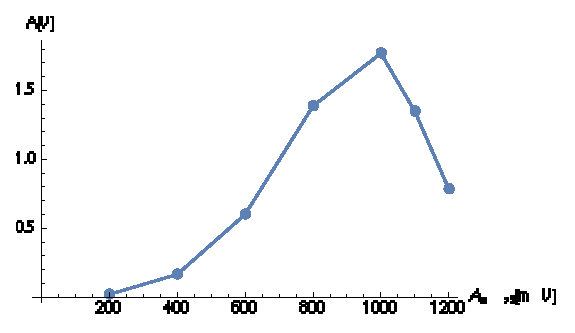
\includegraphics[width=0.45\textwidth]{wykr_AodA1H.eps}
\label{fig:goda1H}
}
\subfigure[]{
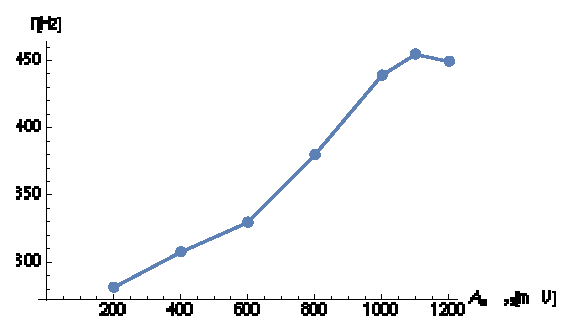
\includegraphics[width=0.45\textwidth]{wykr_GodA1H.eps} 
\label{fig:aoda1H}
}


\subfigure[]{
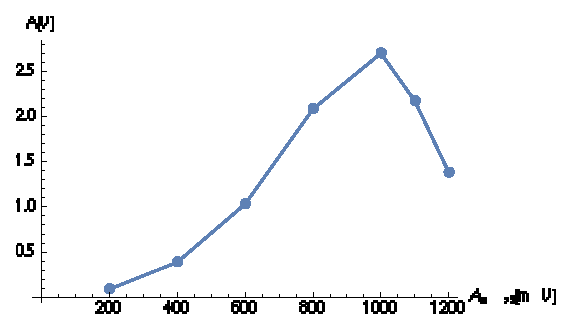
\includegraphics[width=0.45\textwidth]{wykr_AodA2H.eps}
\label{fig:goda1H}
}
\subfigure[]{
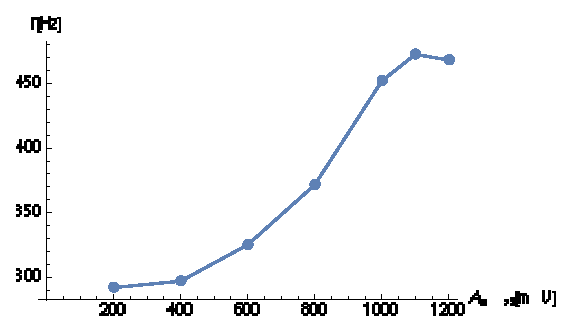
\includegraphics[width=0.45\textwidth]{wykr_GodA2H.eps} 
\label{fig:aoda1H}
}
\caption{ a) Amplituda rezonansu na 1 harmonicznej w zależności od $A_m$ b) Szerokość rezonansu na 1 harmonicznej w zależności od $A_m$ 
c) Amplituda rezonansu na 2 harmonicznej w zależności od $A_m$ d) Szerokość rezonansu na 2 harmonicznej w zależności od $A_m$}
\label{wykresikioda}
\end{figure}


Na rysunku \ref{wykresikiodp} znajduje się zaś zależność powyższych parametrów od od mocy światła padającego na komórkę. Amplituda sygnału magnetorotacji jest wprost proporcjonalna od mocy lasera, ponieważ mierzona jest różnica natężeń światła w dwóch polaryzacjach. Zwiększanie mocy światła powoduje jednak poszerzenie rezonansu.


\begin{figure}[h!]
\centering
\subfigure[]{
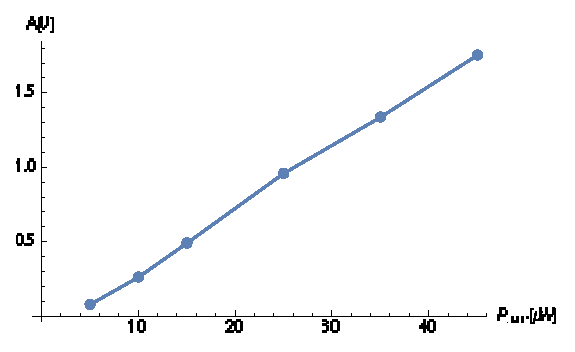
\includegraphics[width=0.45\textwidth]{wykr_AodP1H.eps}
\label{fig:goda1H}
}
\subfigure[]{
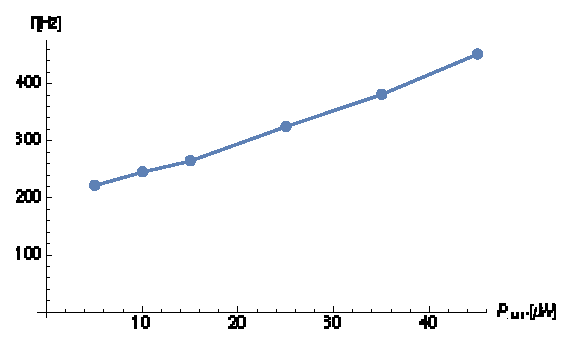
\includegraphics[width=0.45\textwidth]{wykr_GodP1H.eps} 
\label{fig:aoda1H}
}

\subfigure[]{
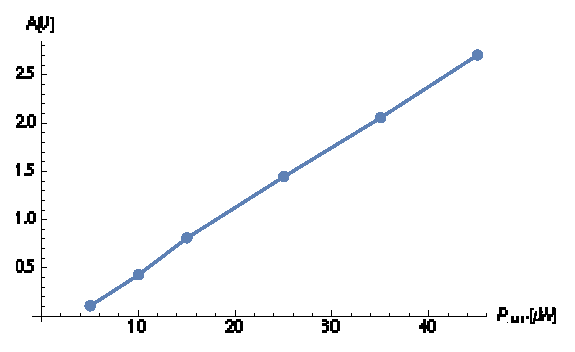
\includegraphics[width=0.45\textwidth]{wykr_AodP2H.eps}
\label{fig:goda1H}
}
\subfigure[]{
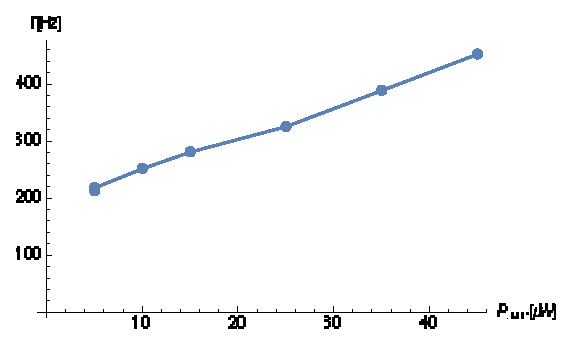
\includegraphics[width=0.45\textwidth]{wykr_GodP2H.eps} 
\label{fig:aoda1H}
}
\caption{ a) Amplituda rezonansu na 1 harmonicznej w zależności od $P_{las}$ b) Szerokość rezonansu na 1 harmonicznej w zależności od $P_{las}$ 
c) Amplituda rezonansu na 2 harmonicznej w zależności od $P_{las}$ d) Szerokość rezonansu na 2 harmonicznej w zależności od $P_{las}$}
\label{wykresikiodP}
\end{figure}

Powyższe pomiary zostały zrobione przy działającym układzie stabilizacji długości fali. Dostrajał on laser do długości fali, przy której sygnał błędu przechodził przez zero (przy przejściu $F=2 \rightarrow F'=2$).

\begin{figure}[h!]
\centering
 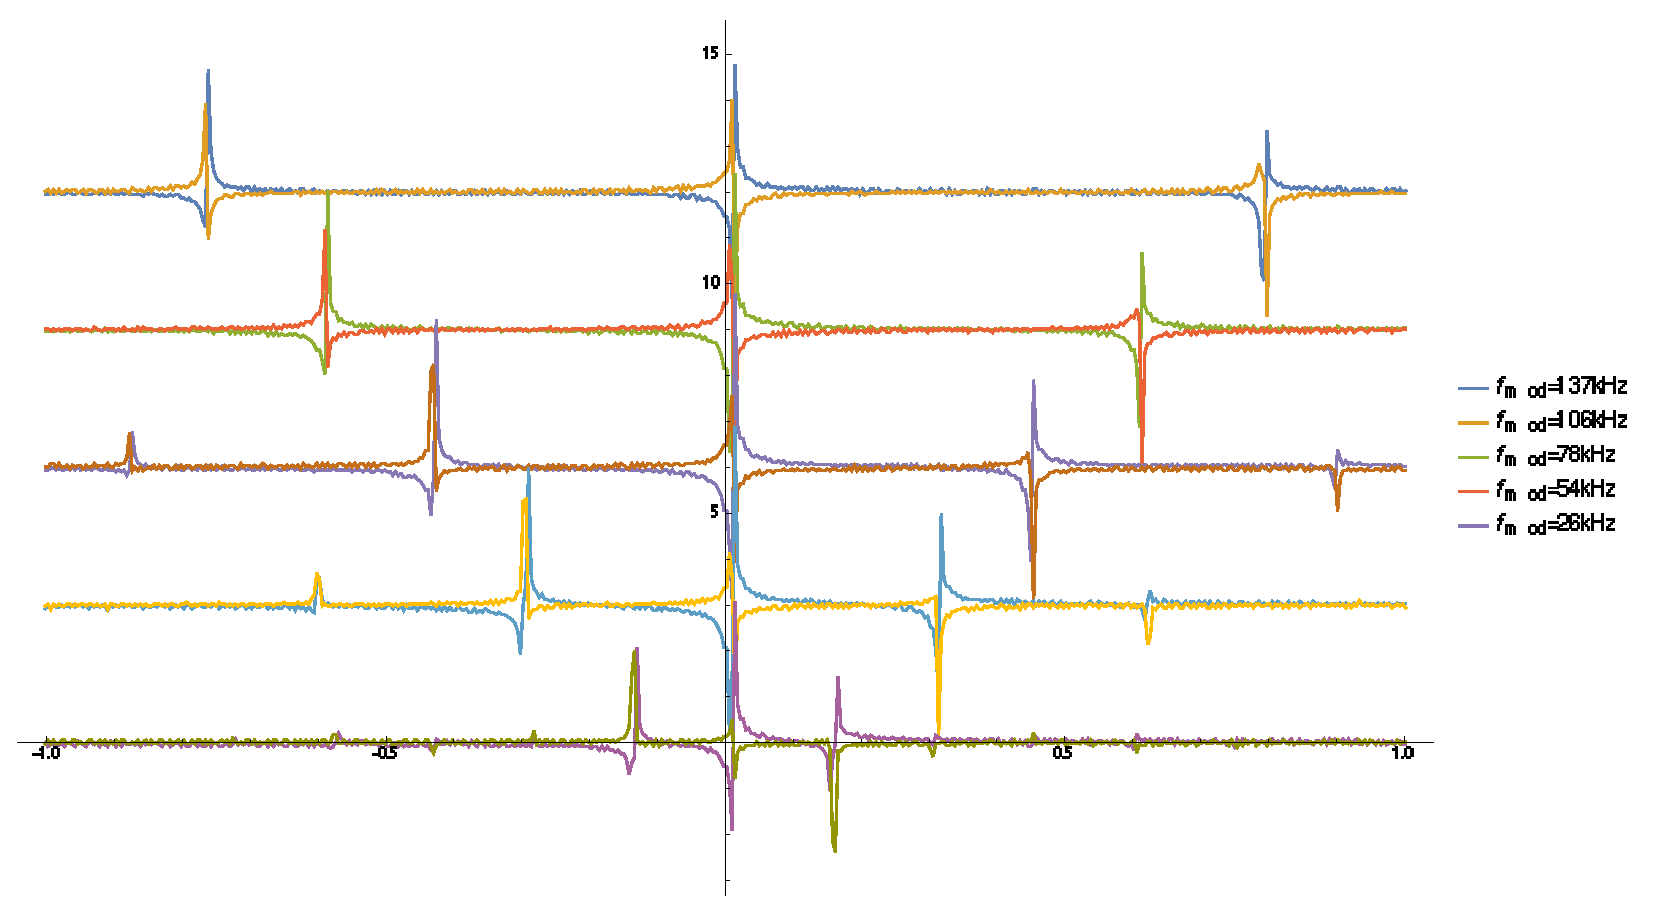
\includegraphics[width=\textwidth]{panoramy_1H_odf.eps}
 % front_all.svg: 1153x455 pixel, 72dpi, 40.68x16.05 cm, bb=0 0 1153 455
 \caption{Zależność magnetorotacji od częstości modulacji. 1 harm. $f_{mod}=101kHz, P_{las}=20 \mu W, A_{mod}=1000mV W$}
 \label{fig:panodf1}
\end{figure}

\begin{figure}[h!]
\centering
 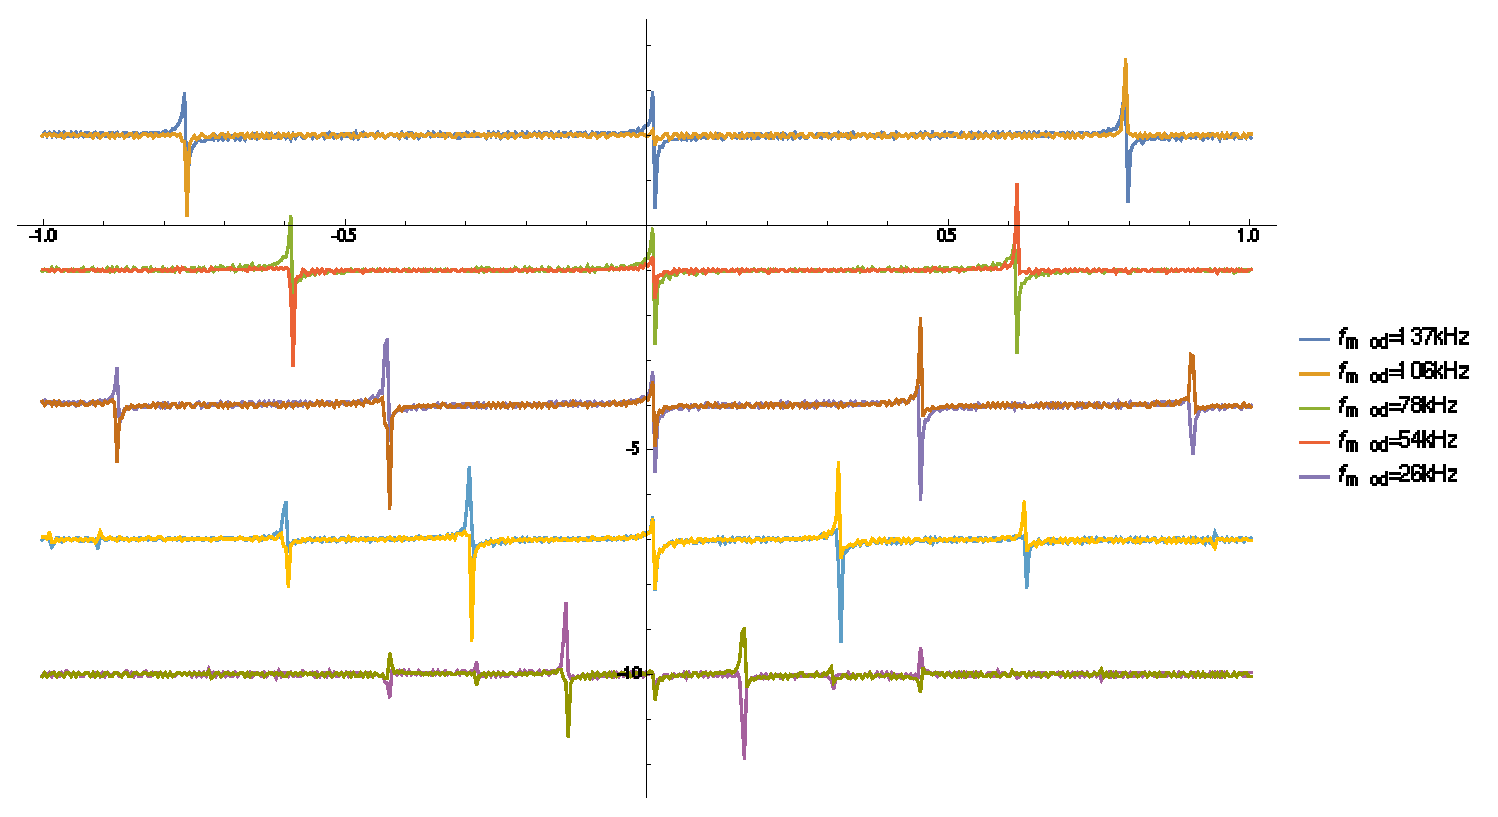
\includegraphics[width=\textwidth]{panoramy_2H_odf.eps}
 % front_all.svg: 1153x455 pixel, 72dpi, 40.68x16.05 cm, bb=0 0 1153 455
 \caption{Zależność magnetorotacji od częstości modulacji. 2 harm. $f_{mod}=101kHz, P_{las}=20 \mu W, A_{mod}=1000mV W$}
 \label{fig:panodf2}
\end{figure}

\begin{figure}[h!]
\centering
 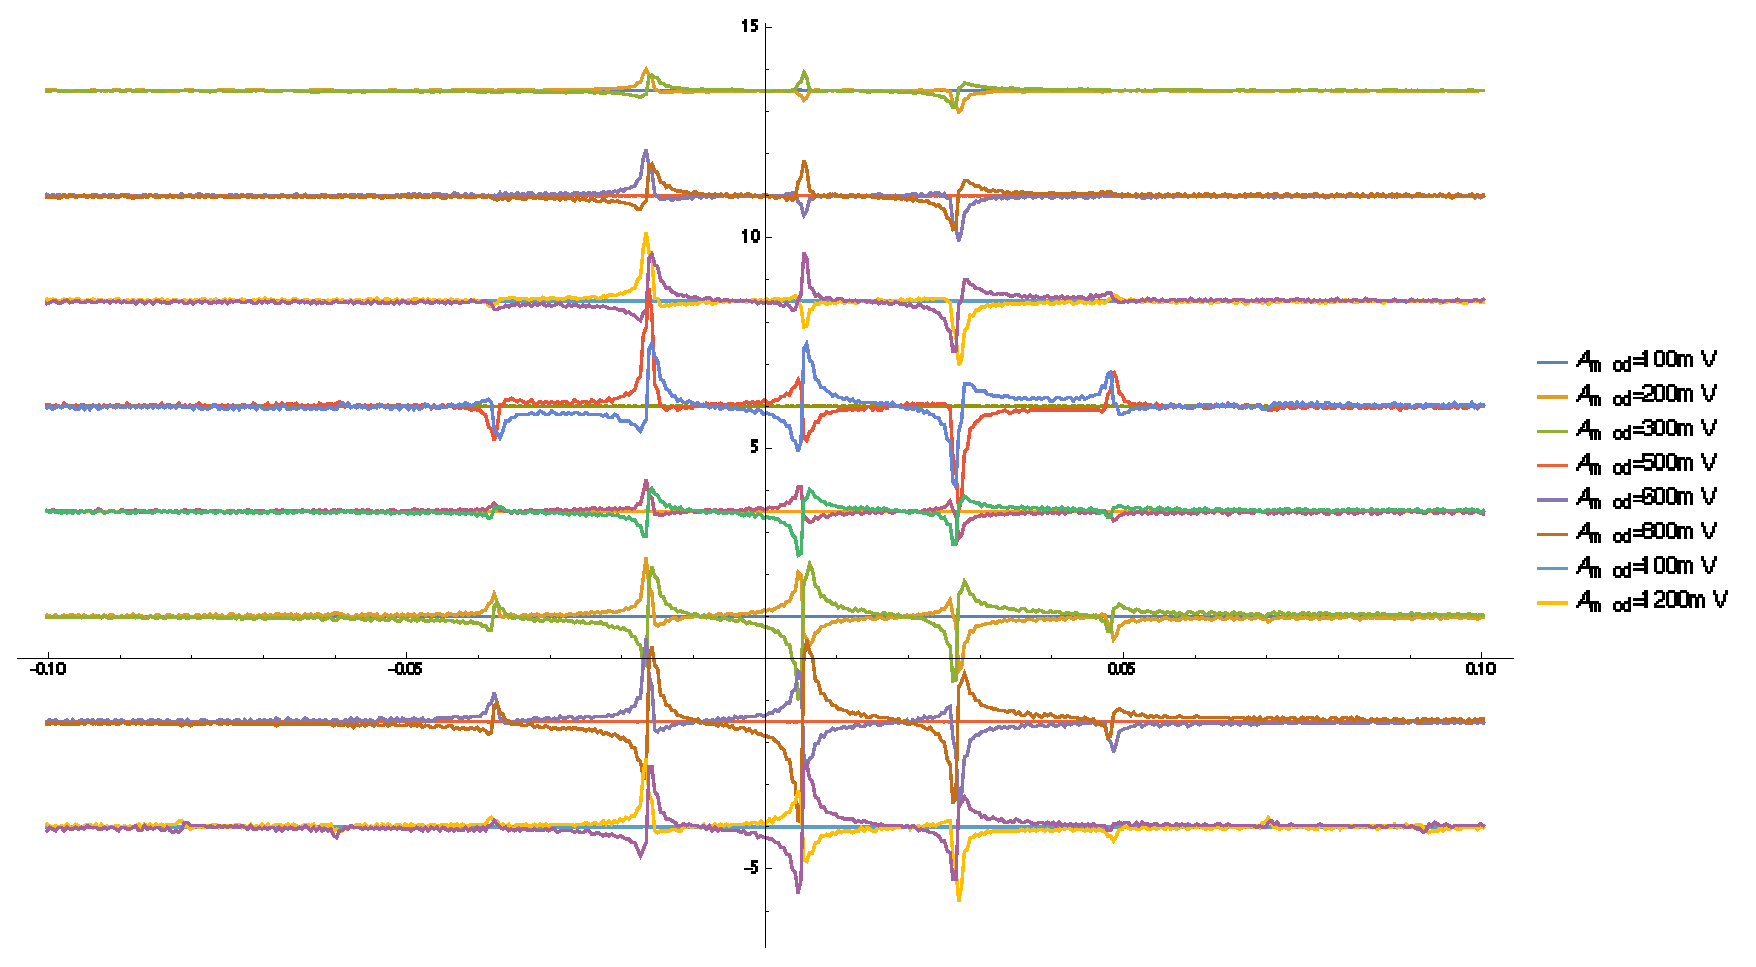
\includegraphics[width=\textwidth]{panoramy_1H_odam.eps}
 % front_all.svg: 1153x455 pixel, 72dpi, 40.68x16.05 cm, bb=0 0 1153 455
 \caption{Zależność magnetorotacji od częstości modulacji. 1 harm. $f_{mod}=101kHz, P_{las}=20 \mu W, A_{mod}=1000mV W$}
 \label{fig:panodam1}
\end{figure}

\begin{figure}[h!]
\centering
 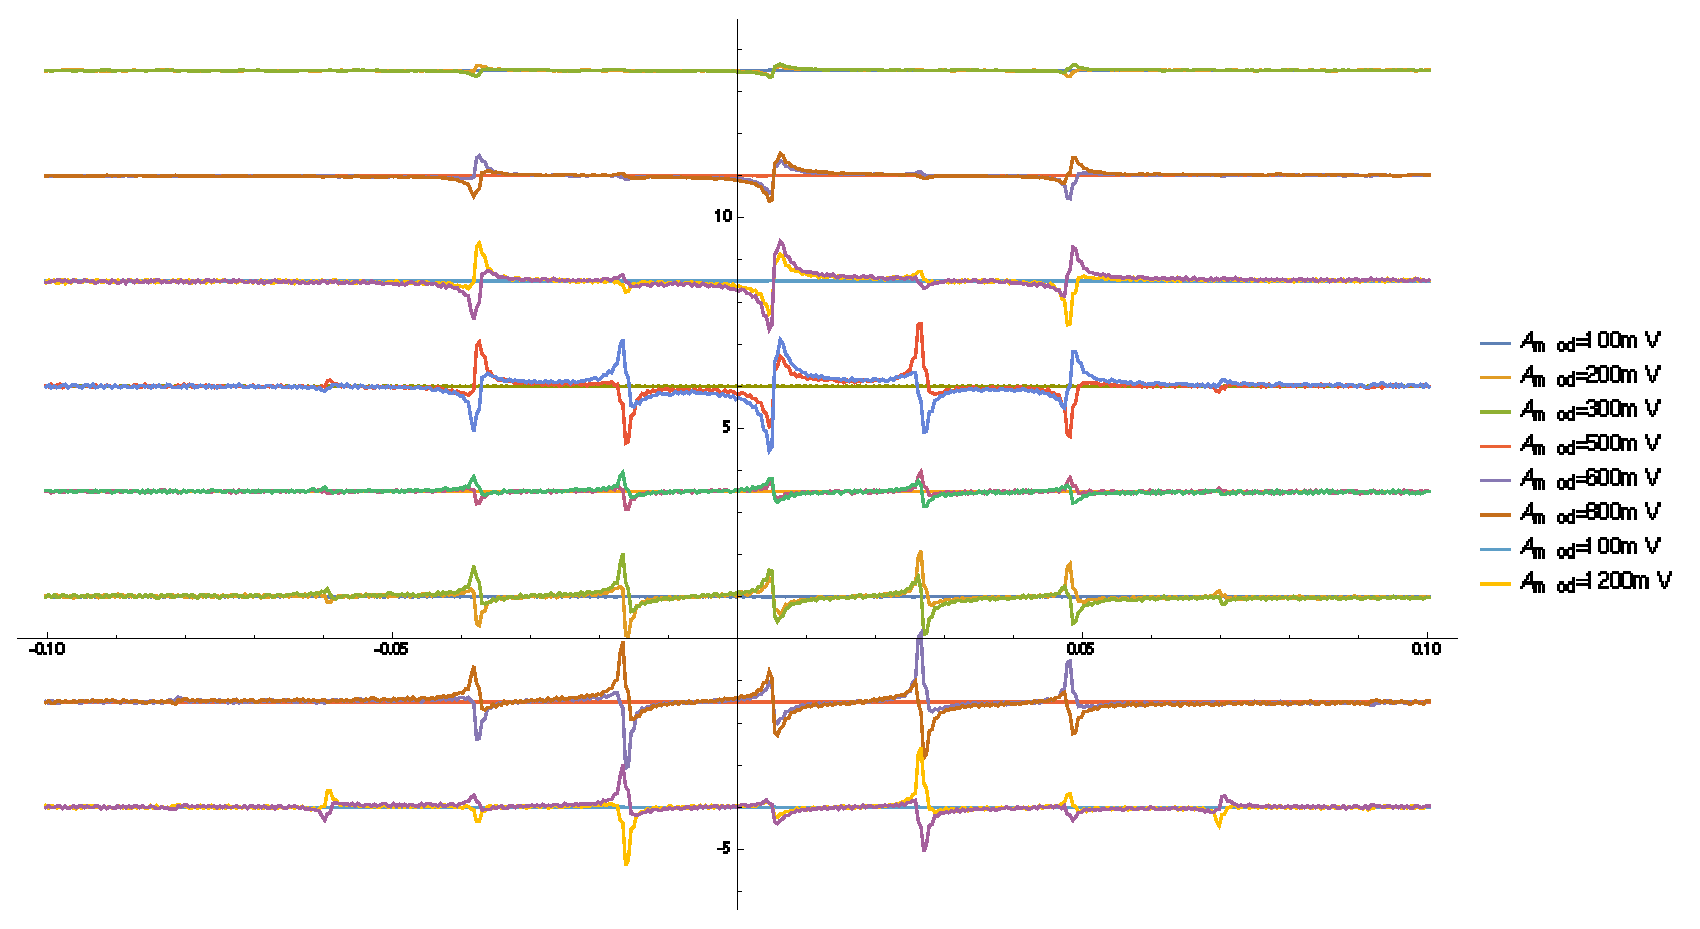
\includegraphics[width=\textwidth]{panoramy_2H_odam.eps}
 % front_all.svg: 1153x455 pixel, 72dpi, 40.68x16.05 cm, bb=0 0 1153 455
 \caption{Zależność magnetorotacji od częstości modulacji. 2 harm. $f_{mod}=101kHz, P_{las}=20 \mu W, A_{mod}=1000mV W$}
 \label{fig:panodam2}
\end{figure}



\begin{thebibliography}{99}
\bibitem{rys-indirect} Goetzberger, Adolf et.al. \emph{Crystalline Silicon Solar Cells}, Chichester: John Wiley \& Sons Ltd., 1998.
\bibitem{rys-laserki} \url{http://wwwold.fi.isc.cnr.it/users/giovanni.giacomelli/Semic/Samples/samples.html}, dostęp 7.12.2015
\bibitem{mgrJustynaMech}  Mech, Justyna \emph{Lasery VCSEL do zastosowań w spektroskopii}, praca magisterska pod kierunkiem Jerzego Zachorowskiego, 2009
\bibitem{steck} Daniel A. Steck, \emph{Rubidium 87 D Line Data, Rubidium 85 D Line Data}~,\url{http://steck.us/alkalidata}
\bibitem{srivansan} R. Srinivasan,\textit{ Nonlinear Magneto-Optical Rotation – A possible tool for sensitive magnetometry}, Current Science \textbf{92}, 298 (2007)

\end{thebibliography}

\end{document}
